\begin{frame}{Weak Scaling}
    Measures scaled speedup when matrix dimension and proseccor count scale togheter.

    \begin{equation*}
        \text{Scaled Speedup} = \frac{N \cdot T_1}{T_N} \quad \text{\footnotesize (Where N is the number of processors)}
        \end{equation*}
    
    \vspace{0.1cm}
    
    
    \begin{figure}[h]
        \centering
        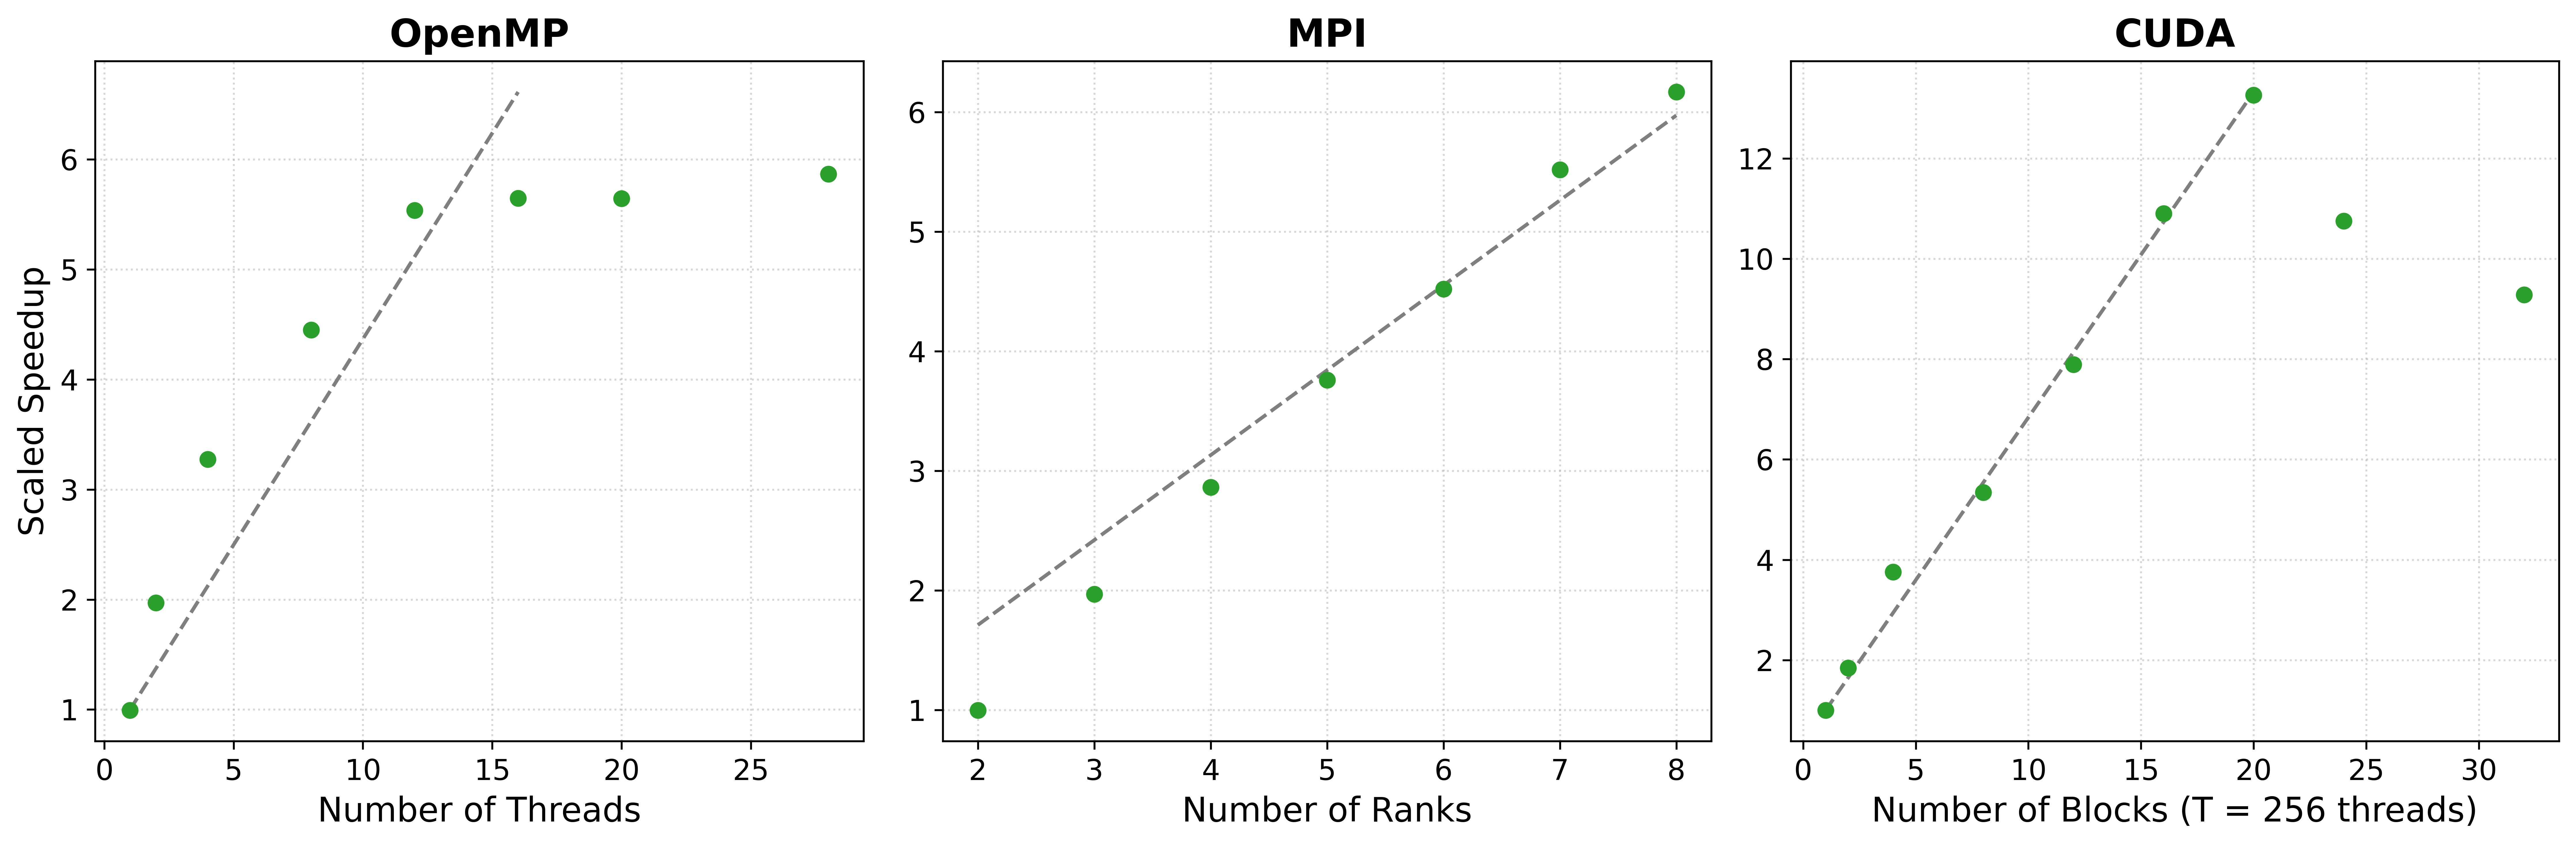
\includegraphics[width=0.99\textwidth]{Images/weak_scaling.png}
        \vspace{-0.2cm}
        \caption{\tiny Points indicate empirical scaled speedup (averaged over 3 runs). Dashed lines illustrate the Gustafson's Law model fit, highlighting parallel overhead scaling limits.}
    \end{figure}
    
    \vfill
    \begin{center}
        \usebeamercolor[fg]{infrastructure}
        \fontsize{6.5pt}{7.5pt}\selectfont
        \texttt{Hardware | WSL2 \quad  CPU: AMD Ryzen 7 8845HS (8C/16T) \quad GPU: NVIDIA RTX 4050 (20 SM)}
    \end{center}
\end{frame}